\documentclass{article}

\usepackage{a4wide}
\usepackage[utf8]{inputenc}
\usepackage[russian]{babel}
\usepackage{graphicx}
\usepackage{amsmath}
\usepackage{amsthm}
\theoremstyle{definition}
\DeclareMathOperator{\sign}{sign}
\usepackage{amsfonts}
\usepackage{amssymb}
\usepackage{subcaption}
\usepackage{indentfirst}
\usepackage{dsfont}
\begin{document}
	
	\thispagestyle{empty}
	
	\begin{center}
		\ \vspace{-3cm}
		
		{\scshape Московский государственный\\
		Ордена Ленина, Ордена Октябрьской Революции,\\
		Ордена Красного Трудового Знамени\\
		университет имени М.~В.~Ломоносова}\\
		Факультет вычислительной математики и кибернетики\\
		Кафедра системного анализа
		
		%\vfill
		\vspace{1cm}
		\begin{center}
		{\includegraphics[width=6cm]{mgu}}
		\end{center}
		\vspace{1cm}
		
		{\LARGE Отчёт по практикуму на ЭВМ}
		
		\vspace{1cm}
		
		{\Huge\bfseries <<Построение множества достижимости>>}
		\end{center}
		
		\vspace{1cm}
		
		\begin{flushright}
		  \large
		  \textit{Студент 315 группы}\\
		  А.\,А.~Самойлов
		
		  \vspace{5mm}
		
		  \textit{Руководитель практикума}\\
		  к.ф.-м.н., доцент П.\,А.~Точилин
		\end{flushright}
		
		\vspace{5cm}
		
		\begin{center}
		  2021
		\end{center}
		
		\newpage
	
	\newpage
	\tableofcontents
	\newpage
	{\vspace*{-2cm} \hspace*{-1cm}\section{Постановка задачи}}
	{Задано обыкновенное дифференциальное уравнение:}
	\begin{equation}
		\ddot x + x^2 + \sin(\dot x) + x\sin^2(x^3) = u,
	\end{equation}  
	{где $x \in \mathbb{R}, u \in \mathbb{R}.$ На возможные значения управляющего параметра наложено ограничение: $u \in [-\alpha, \alpha].$ Задан начальный момент времени $t_0 = 0$ и начальная позиция $x(t_0) = 0, \dot x(t_0) = 0.$ Необходимо построить множество достижимости $X(t,t_0,x(t_0),\dot x(t_0))$ (множество пар $(x(t), \dot x(t))$) в классе программируемых управлений в заданный момент времени $t \geq t_0$.}
	\begin{itemize}
		\item [1)]{Необходимо написать в среде MatLab функцию reachset(alpha,t), которая по заданным параметрам $\alpha > 0, t \geq t_0$ рассчитывает приближенно множество достижимости $X(t,t_0,x(t_0), \dot x(t_0)).$ На выходе функции --- два массива $X,Y$ с упорядоченными координатами точек многоугольника, образующего границу искомого множества. Точки в этих массивах должны быть упорядочены так, чтобы результаты работы функции без дополнительной обработки можно было подавать на вход функциям визуализации (например, plot). Предусмотреть такой режим работы функции, при котором она возвращает также координаты линий переключений оптимального управления (с возможностью их визуализации).}
		\item [2)]{Необходимо реализовать функцию reachsetdyn(alpha,t1,t2,N,filename), которая, используя функцию reachset(alpha,t), строит множества достижимости для моментов времени $\tau_i = t_1 + \frac{(t_2 - t_1)^i}{N}, i = 0,1,\ldots, N$. Здесь $t_2 \geq t_1 \geq t_0, N$--- натуральное число. Для каждого момента времени $\tau_i$ функция должна отобразить многоугольник, аппроксимирующий границу множества достижимости. Результат работы функции (анимация изменения границы множества достижимости) должен быть сохранен в виде видео-файла filename.avi. Необходимо также предусмотреть вариант работы функции (при отсутствии параметра filename) без сохранения в файл, с выводом непосредственно на экран. Как частный случай, функция должна иметь возможность строить границу множества достижимости в один фиксированный момент времени ($t_2 = t_1$).}
		\item [3)]{В соответствующем задании отчете необходимо привести все теоретические выкладки, сделанные в ходе построения множества достижимости, описать схему алгоритма построения множества достижимости программой, привести примеры построенных множеств достижимости (с иллюстрациями), исследовать зависимость множеств достижимости от величины параметра $\alpha$. Все вспомогательные утверждения (за исключением принципа максимума Понтрягина), указанные в отчете, должны быть доказаны.}
	\end{itemize}
	
	\newpage
	{\vspace*{-2cm} \hspace*{-1cm}\section{Теоретические выкладки}}
	{Проведем замену переменных $x_1 = x;  x_2 = \dot x.$ Получим систему:}
	\begin{equation}
		\begin{cases}
		\dot x_1 = x_2,\\
		\dot x_2 = u - x_1^2 - \sin(x_2) - x_1\sin^2(x_1^3),\\
		x_1(0) = 0,\\
		x_2(0) = 0.
		\end{cases}
	\end{equation}
	
	{Введем функцию Гамильтона-Понтрягина: }
	\begin{equation}
	H(\psi, x, u) = \langle \psi, f(x,u) \rangle.
	\end{equation}
	{\textbf{Определение 1} \textit{Множество достижимости} $X(t,t_0,x^0)$ --- множество концов траектории системы
	\begin{equation}
		\begin{cases}
		\dot x(t) = f(t,x(t),u(t)),\\
		u(t) \in U(t),\\
		x(t_0) = x^0,\\
		\end{cases}
	\end{equation}
	
	при любом допустимом управлении.}

 	\newtheorem{theorem}{Теорема}
 	\begin{theorem}
 		\textit{(Принцип максимума Понтрягина)}

		Рассмотрим систему:
 		\begin{equation}
 		\dot x = f(x,u),
 		\end{equation}
 		
 		{заданную в $\mathbb{R}^n,$ где $f(x,u), \frac{\partial f}{\partial x}(x,u)$--- непрерывные функции, определенные на $\mathbb{R}^{n}.$ Пусть $U$~--- множество допустимых управлений на интервале $0 \leq t \leq T,$ удовлетворяющих ограничению $u(t) \in \mathcal{P} \in \mathbb{R}^m$. Пусть некоторому допустимому управлению $u^*(t) \in U$ соответствует решение $x^*(t)$ с концом $x^*(T)$, лежащим на границе множества достижимости. Тогда существует ненулевое сопряженное решение $\psi^*(t)$ системы}
 		\begin{equation}
 		 \dot \psi = - \langle \psi, \frac{\partial f}{\partial x}(x^*,u^*) \rangle
 		\end{equation}
 		
 		{такое, что почти всюду выполняется принцип максимума:}
 		\begin{equation}
 			H(\psi, u^*, x^*) = \sup \limits_{u \in \mathcal{P}} H(\psi, u, x).
 		\end{equation}
 		
 		{Если управление $u^*(t)$ ограничено, то:}
 		\begin{equation}
 			\sup \limits_{u \in \mathcal{P}}H(\psi, u, x) = const \geq 0, \text{для п.в. } t \in [0, T].
 		\end{equation}
	\end{theorem}
 		
	{Для нашей системы функция Гамильтона-Понтрягина имеет вид:}
	\begin{equation}
		H(\psi, u , x) = \psi_1x_2 + \psi_2u - \psi_2x_1^2 - \psi_2\sin(x_2) - \psi_2x_1\sin^2(x_1^3).
	\end{equation}
	
	{Выпишем сопряженную систему:}
	\begin{equation}
		\begin{cases}
	\dot \psi_1 = 2\psi_2x_1 + \psi_2\sin^2(x_1^3) + 6\psi_2x_1^3\cos(x_1^3)\sin(x_1^3);\\
	\dot \psi_2 = -\psi_1 + \psi_2\cos(x_2);
	\end{cases}
	\end{equation}
 	
 	{Поэтому, если точка принадлежит границе множества достижимости, то она удовлетворяет принципу максимума Понтрягина. Для построения границы множества достижимости построим все траектории, удовлетворяющие принципу максимума. }
 	\newpage
 	{Из принципа максимума следует, что $u^*(t) = \alpha\sign(\psi_2(t)),$ а переключения происходят в момент времени $\psi_2(t) = 0.$}
 	\newline
 	{Сформулируем две теоремы о нулях $\psi_2(t):$}
 	\begin{theorem}
 		{(О конечном числе нулей) Пусть $u(t)$~--- оптимальное управление для исходной системы, тогда $\psi_2(t)$ имеет конечное число нулей на отрезке $[0, T].$}
 		
    \end{theorem}	
 		{\textbf{Доказательство:} Пусть на  конечном интервале времени $\psi_2(t)$ имеет бесконечное число нулей, тогда (так как интервал времени конечен) существует такой момент времени $t^*$(точка "накопления"), в который $\psi_2(t^*) = 0$ и $\dot \psi_2(t^*) = 0.$ Тогда $\dot \psi_1(t^*) = 0$ и $\psi_1(t^*) = 0$, что противоречит тому, что вектор $\psi(t)$ ненулевой.} 
 	
 
 	\begin{theorem}
 		{(О чередовании нулей) Пусть $(x(\cdot), u(\cdot))$--- оптимальная пара с временем быстродействия $T, \psi(\cdot)=(\psi_1(\cdot),\psi_2(\cdot))$ --- решение сопряженной системы. Тогда $\forall \tau_1, \tau_2: 0 < \tau_1 < \tau_2 < T$ справедливы следующие утверждения:}
 		\begin{itemize}
 			\item [1.]{Если $\psi_2(\tau_1)=\psi_2(\tau_2)=0$ и $x_2(\tau_1)=0,$ тогда $x_2(\tau_2)=0.$}
 			\item [2.]{Если $\psi_2(\tau_1)=\psi_2(\tau_2)=0$ и $x_2(\tau_1)\neq 0,$ но $\exists \tilde{\tau} \in [\tau_1, \tau_2]:x_2(\tilde{\tau})=0. $}
 			\item [3.]{Если $x_2(\tau_1) = x_2(\tau_2)=0, x_2(\tau) \neq 0, \forall \tau \in (\tau_1, \tau_2)$ и $\psi_2(\tau_1)=0$, тогда $\psi_2(\tau_2)=0.$}
 			\item [4.]{Если $x_2(\tau_1) = x_2(\tau_2)=0, x_2(\tau) \neq 0, \forall \tau \in (\tau_1, \tau_2)$ и $\psi_2(\tau_1)\neq0$, тогда $\psi_2(\tau_2)\neq0,$ но $\exists \tilde{\tau}\in [\tau_1, \tau_2]:\psi_2(\tilde{\tau})=0.$}
 		\end{itemize}
 	\end{theorem}
 	{\textbf{Доказательство:}}
 	\begin{itemize}
 		\item [1.]{Применим (7) для моментов времени $\tau_1,\tau_2,$ получим $\psi_1(\tau_1)x_2(\tau_1)=\psi_1(\tau_2)x_2(\tau_2).$ $x_2(\tau_1)=0 \Rightarrow \psi_1(\tau_2)x_2(\tau_2) = 0,\psi_2(\tau_2)$ по условию равно 0, а так как вектор $\psi(\cdot)$ ненулевой, то $\psi_1(\tau_2) \neq 0 \Rightarrow x_2(\tau_2) = 0.$}
 		\item [2.]{$\psi_1(\tau_1)x_2(\tau_1) = \psi_1(\tau_2)x_2(\tau_2).$ Так как $x_2(\tau_1) \neq 0, \psi_1(\tau_1)\psi_1(\tau_2) < 0,$ то $x_2(\tau_1)x_2(\tau_2) < 0,$ что значит, что $x_2(\tau)$ имеет единственный корень на $[\tau_1,\tau_2]$ ~--- $\tilde{\tau}.$} 
 		\item [3.]{Из пункта 1 имеем, что $\psi_2(\tau) \neq 0, \tau \in (\tau_1, \tau_2).$ Тогда: 
 		\begin{equation}
 			 \frac{d}{dt}(x_2\psi_1 + \dot{x}_2\dot{\psi}_2) = 0 = \dot{x}_2\psi_1 + x_2\frac{\partial f}{\partial x_1}\psi_2 + \ddot{x}_2\psi_2 + \dot{x}_2(-\psi_1 + \psi_2\frac{\partial f}{\partial x_2})
 		\end{equation}
 		\begin{equation}
 			\dot{x}_2(\tau_1)\psi_2(\tau_1) = \dot{x}_2(\tau_2)\psi_2(\tau_2).
 		\end{equation}
 		Так как $\psi_2(\tau_1) = 0,$ а $x_2(\tau_2) \neq 0$ (иначе система имела бы только тривиальное решение). Поэтому $\psi(\tau_2) = 0.$
 	 }
 		\item [4.]{Так как $\psi_2(\tau_1) \neq 0,$ то $\psi_2(\tau_2) \neq 0.$ Если $\psi_2(\tau)$ не обращается в ноль на $[\tau_1, \tau_2],$ то $\dot{x}_2(\tau_1)\dot{x}_2(\tau_2) > 0,$ что противоречит тому, что $\tau_1, \tau_2$ --- последовательные корни $x_2$ $\Rightarrow \exists \tilde{\tau} \in [\tau_1, \tau_2]:\psi_2(\tilde{\tau}) = 0$ }
 	\end{itemize}
 	
 	{Из теоремы следует, что либо нули $x_2$ и $\psi_2$ совпадают, либо они чередуются. Без ограничения общности будем считать, что $\psi_1 = 1$. Разобьем систему (2) на две:}
 	\begin{equation}
 		S_+ : \begin{cases}
 		\dot{x}_1 = x_2\\
 		\dot{x}_2 =  \alpha - x_1^2 - \sin(x_2) - x_1\sin^2(x_1^3)
 		\end{cases}
 	\end{equation}
 	\begin{equation}
 		S_- : \begin{cases}
 		\dot{x}_1 = x_2\\
 		\dot{x}_2 =  -\alpha - x_1^2 - \sin(x_2) - x_1\sin^2(x_1^3)
 		\end{cases}
 	\end{equation}
 	{Система $S_+$ отвечает управлению $\alpha$, система $S_-$--- $-\alpha.$ }
 	\newline
 	{Пусть сначала управление равно $\alpha$, тогда решаем систему $S_+$ и находим момент времени $t^*:x_2(t^*)=0.$ Построим траекторию, соответствующую системе $S_+$ до момента времени $t^*$. Из теоремы 3 мы знаем, что нули $\psi_2$ чередуются с нулями $x_2$. Организуем перебор по равномерной сетке на отрезке $[0; t^*]$ времени переключения $\hat{t}$. В момент переключения $\hat{t}$ управление станет равно $-\alpha.$ Тогда будем строить траекторию из точки $(x_1(\hat{t}),x_2(\hat{t}))),$ соответствующую системе $S_-$ до нового момента переключения, который находится из решения сопряженной системы с начальными условиями:}
 	\begin{equation}
 	\begin{cases}
  	\psi_1(\hat{t}) = 1,\\
 	\psi_2(\hat{t}) = 0.
 	\end{cases}
 	\end{equation}
 	{Такой выбор начальных условий связан с нормировкой вектора $\psi$. Процесс продолжается ($u = \alpha$) меняется на ($u = -\alpha$) пока $t < T.$ Для системы с начальным управлением $-\alpha$ процесс полностью аналогичен.}
 	{\section{Алгоритм решения}}
 	\begin{itemize}
 		\item [1.]{Решить систему $S_+$, получить момент времени $t^*: x_2(t^*) = 0.$}
 		\item [2.]{Сделать перебор по времени переключения на отрезке $[0;t^*]$.}
 		\item [3.]{Решить сопряженную систему с начальными условиями (14) и систему $S_-,$ найти момент времени $t:\psi_2(t) = 0.$}
 		\item [4.]{Если $t < T$ сделать переключение и решать систему $S_+,$ а сопряженную систему с условиями $[-1;0].$}
 		\item [5.]{Повторять до $t \geq T.$}
 		\item [6.]{Аналогично поступить с системой $S_-$ при начальном $u = -\alpha.$}
 		\item [7.]{Объединить полученную кривую в общее целое, которое и является границей множества достижимости. }
 		\item [8.]{При построении каждой траектории координаты точек переключения добавляются в специальный массив, а затем объединяются в кривую переключений.}
 	\end{itemize}
 	
 	\newpage
 	{\section{Иллюстрация работы программы}}
 	\begin{center}
 		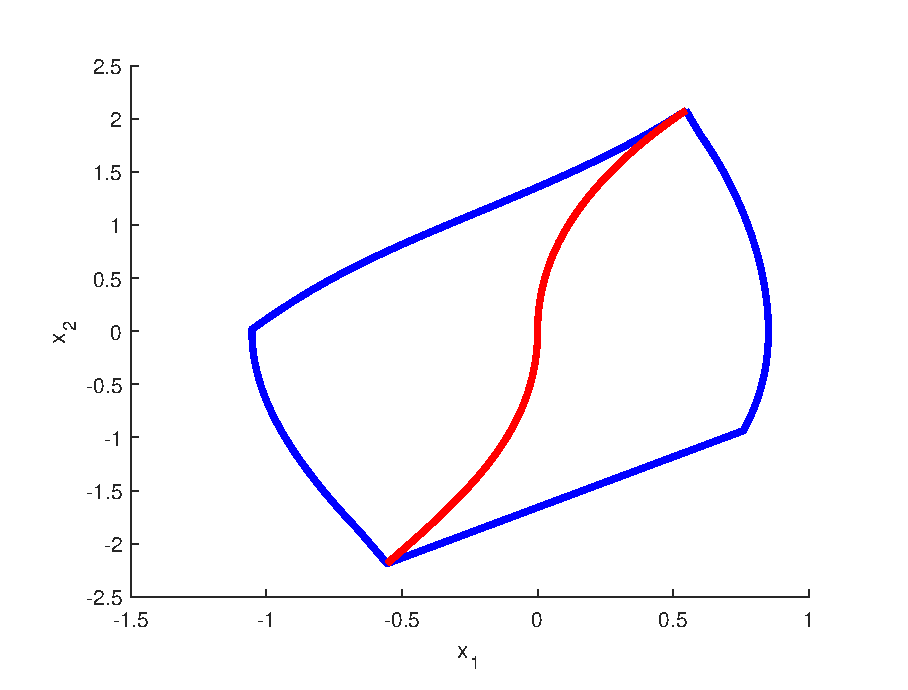
\includegraphics[width=0.7\textwidth]{example1.eps}\\
 		{Рис. 1. Аппроксимация множества достижимости при $\alpha = -5, t = 0.5$ }
 	\end{center}
 
	\begin{center}
		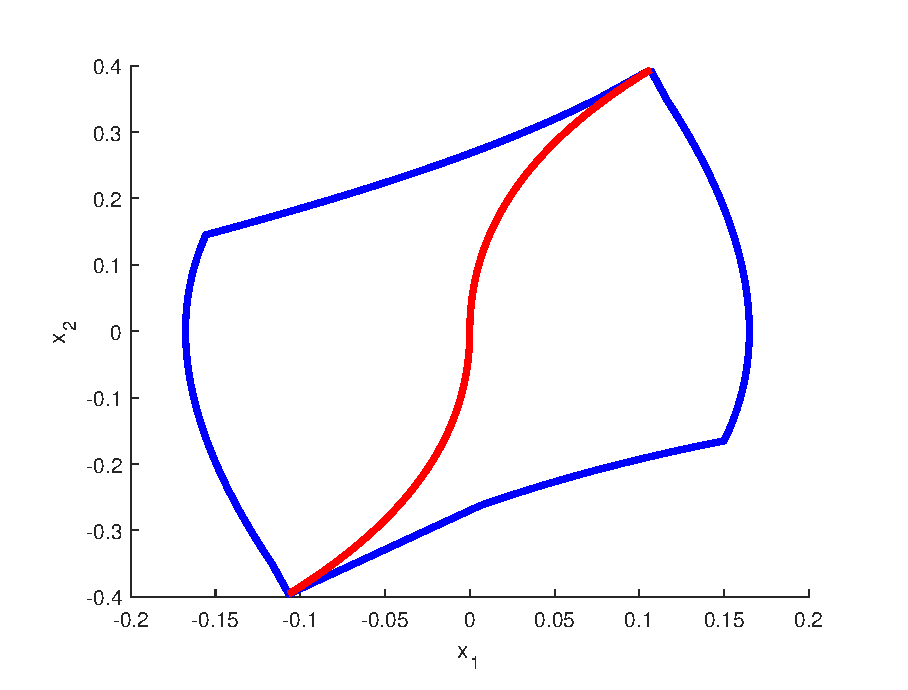
\includegraphics[width=0.7\textwidth]{example2.eps}\\
		{Рис. 2. Аппроксимация множества достижимости при $\alpha = -1, t = 0.5$ }
	\end{center}

	\begin{center}
		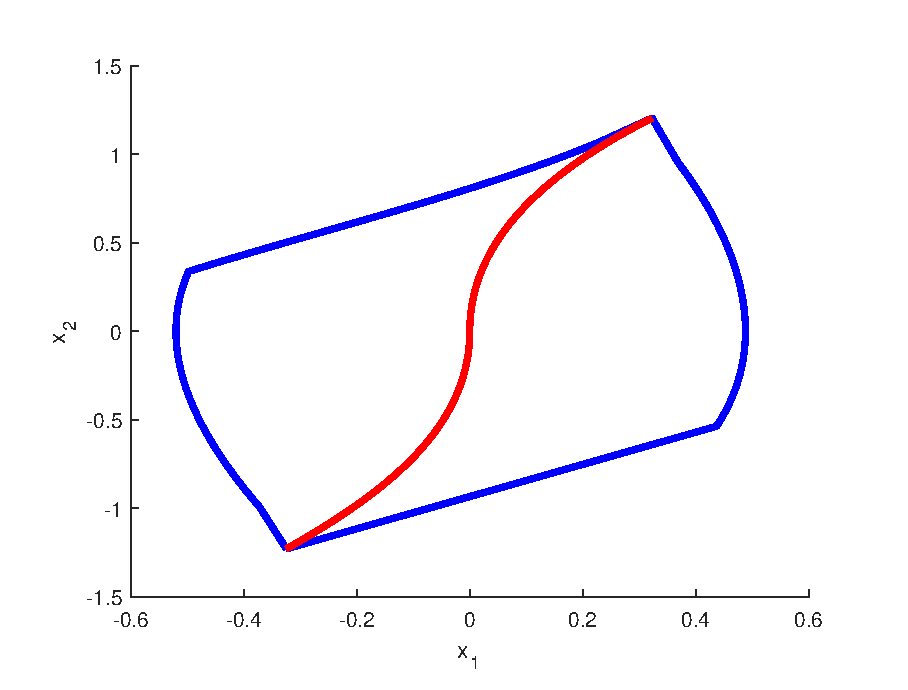
\includegraphics[width=0.7\textwidth]{example3.eps}\\
		{Рис. 3. Аппроксимация множества достижимости при $\alpha = 3, t = 0.5$ }
	\end{center}

	\begin{center}
		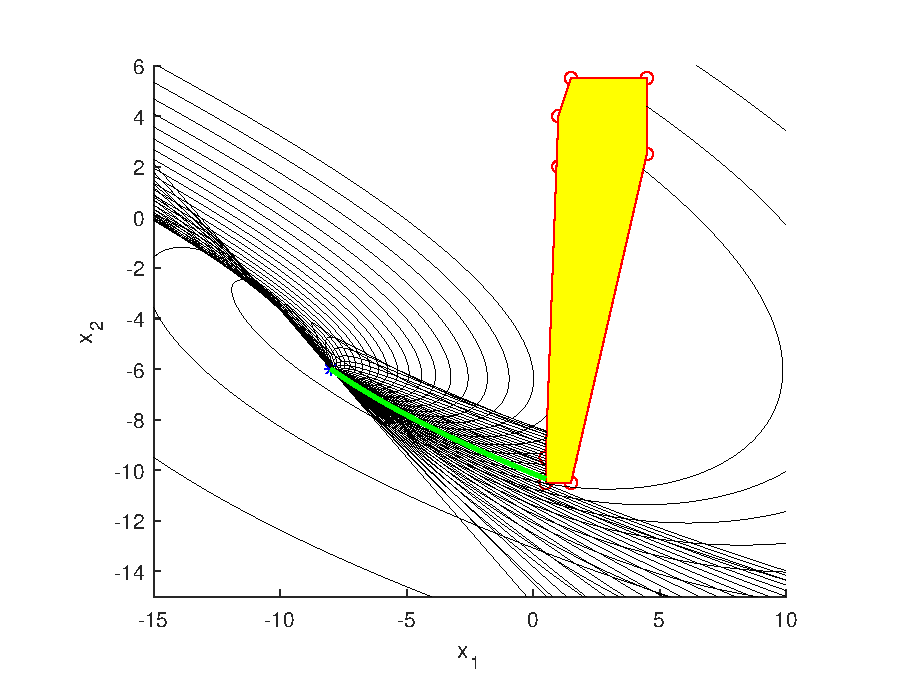
\includegraphics[width=0.7\textwidth]{example4.eps}\\
		{Рис. 4. Аппроксимация множества достижимости при $\alpha = 5, t = 0.5$ }
	\end{center}
	\begin{center}
		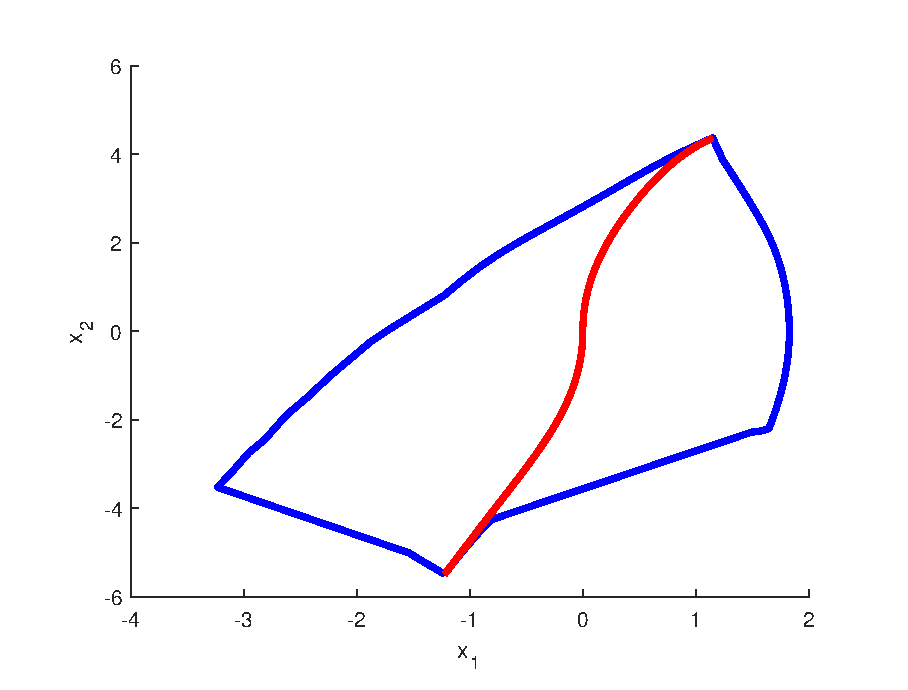
\includegraphics[width=0.7\textwidth]{example5.eps}\\
		{Рис. 5. Аппроксимация множества достижимости при $\alpha = 10, t = 0.5$ }
	\end{center}
	\begin{center}
		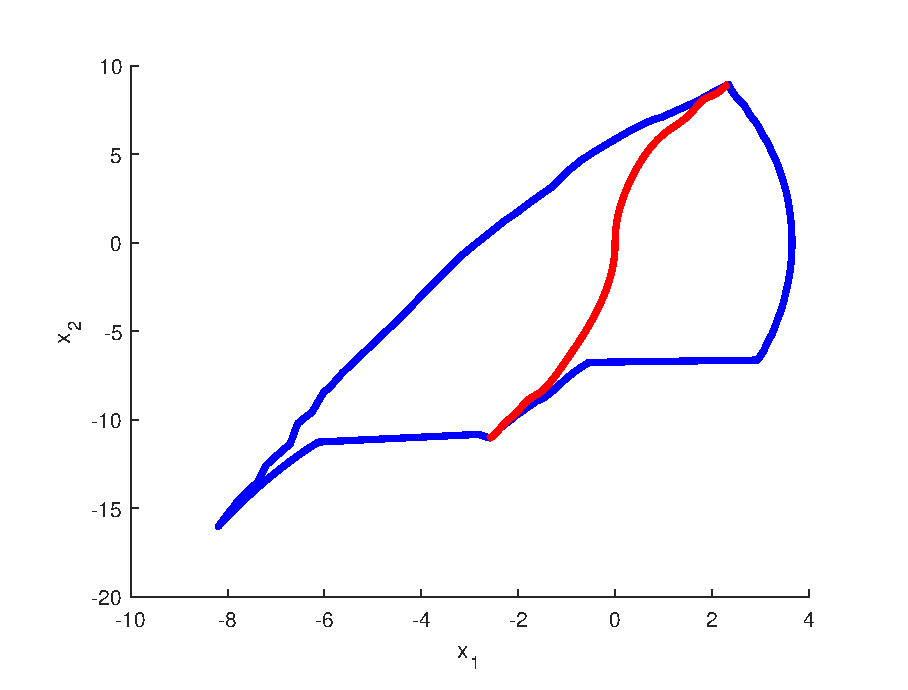
\includegraphics[width=0.7\textwidth]{example6.eps}\\
		{Рис. 6. Аппроксимация множества достижимости при $\alpha = 20, t = 0.5$ }
	\end{center}
	{Как можно заметить по графикам, при увеличении параметра $\alpha$ происходит увеличение множества достижимости.}
	\newpage
	{\subsection{Изменение множества достижимости с течением времени}}
	\begin{center}
		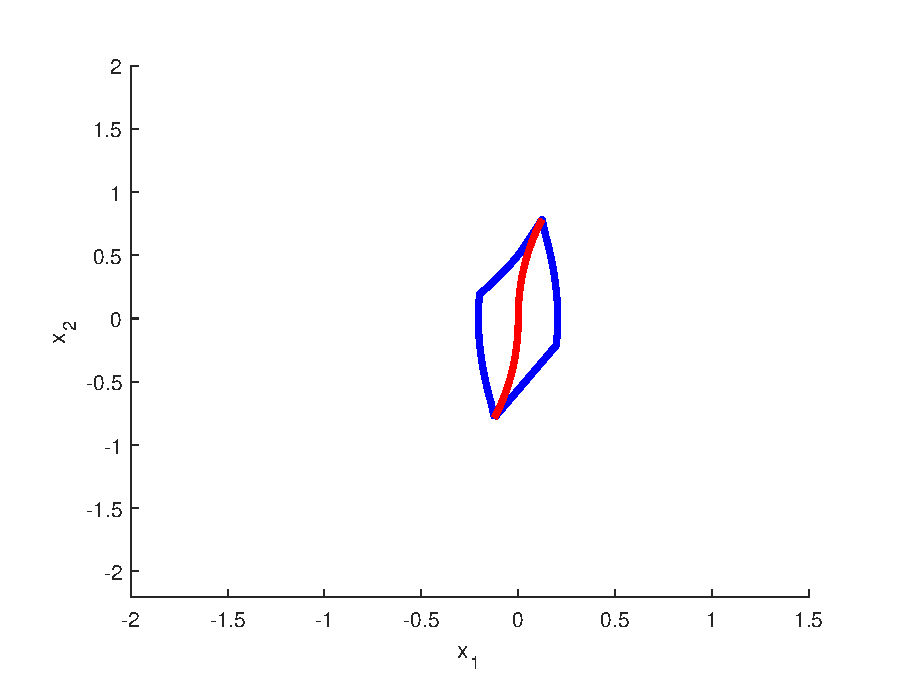
\includegraphics[width=0.7\textwidth]{texample1.eps}\\
		{Рис. 7. Аппроксимация множества достижимости при $\alpha = 3, t = 0.3$ }
	\end{center}
	\begin{center}
		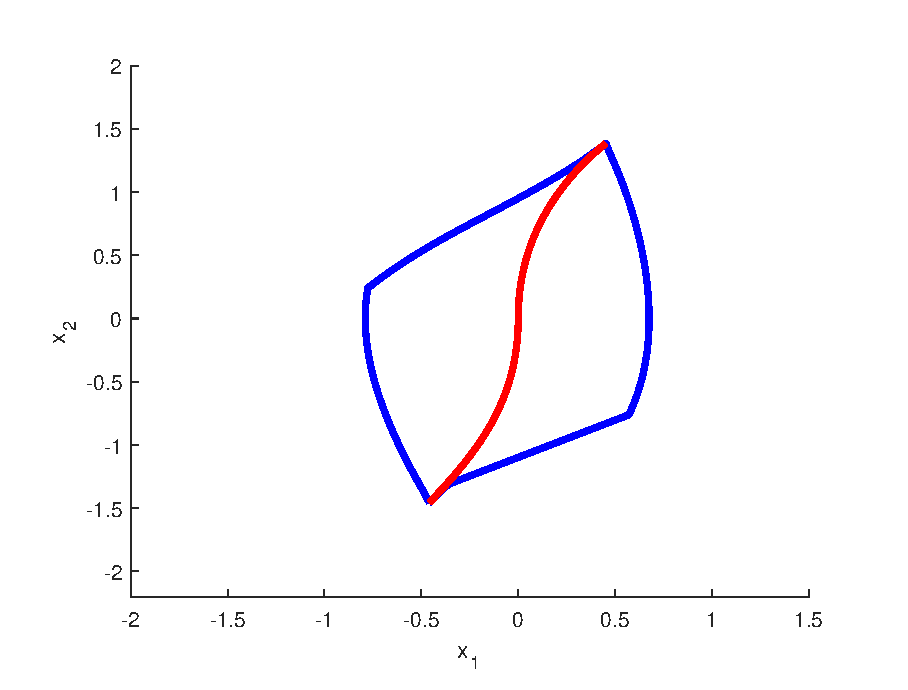
\includegraphics[width=0.7\textwidth]{texample2.eps}\\
		{Рис. 8. Аппроксимация множества достижимости при $\alpha = 3, t = 0.6$ }
	\end{center}
	\begin{center}
		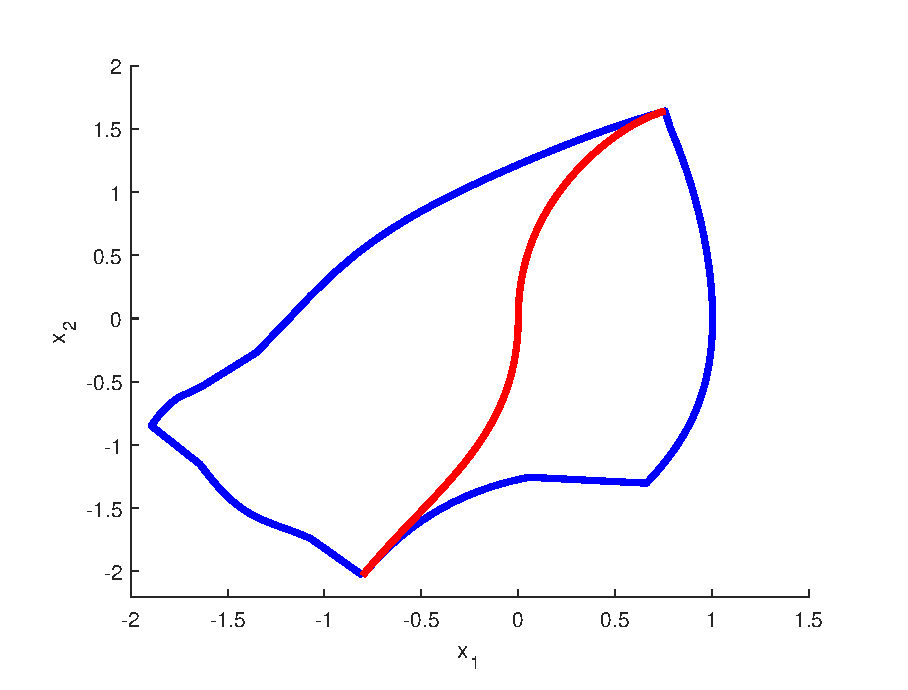
\includegraphics[width=0.7\textwidth]{texample3.eps}\\
		{Рис. 9. Аппроксимация множества достижимости при $\alpha = 3, t = 0.8$ }
	\end{center}
	\newpage
	\newpage
\begin{thebibliography}{9}
  \bibitem{lektures} Ли Э.Б., Маркус Л. \emph{Основы теории оптимального управления}.
  \bibitem{OC} Л.С. Понтрягин, В.Г. Болтянский, Р.В. Гамкрелидзе, Е.Ф. Мищенко \emph{Математическая теория оптимальных процессов}.
  \bibitem{lektures} Комаров Ю. \emph{Лекции по курсу оптимальное управление}.
\end{thebibliography}

\end{document}	